\section{实验}


我们使用 MNIST 和 Frey Face 数据集\footnote{可从\url{http://www.cs.nyu.edu/~roweis/data.html}获取。}中的图像训练生成模型，并通过变分下界与估计的边缘似然比较不同学习算法。

采用第\ref{sec:example}节的生成模型（解码器）和变分近似（编码器），其中编码器与解码器的隐藏单元数相同。由于 Frey Face 数据是连续的，我们采用高斯输出的解码器，其结构与编码器相同，只是在解码器输出端使用 sigmoid 激活函数，将均值限制在 $(0,1)$ 内。
注意，\emph{隐藏单元}指编码器和解码器神经网络中的隐藏层单元。

参数通过随机梯度上升更新。梯度由对下界估计量求导得到，即 $\nabla_{\bT,\bphi}\LBT{M}{\bX^M}$（见算法\ref{algorithm}），并加入一个较小的权重衰减项，对应于先验 $p(\bT)=\mathcal{N}(0,\bI)$。优化该目标相当于近似 MAP 估计，其中用下界梯度近似对数似然梯度。

我们比较了 AEVB 与唤醒—睡眠算法\cite{hinton1995wake}的性能。两者采用相同的编码器，也称识别模型。所有变分参数和生成参数都从 $\mathcal{N}(0,0.01)$ 随机采样初始化，并按 MAP 准则联合进行随机优化。步长使用 Adagrad\cite{duchi2010adaptive}自适应调整；其全局步长参数根据最初几轮迭代在训练集上的表现，从 $\{0.01,0.02,0.1\}$ 中选择。minibatch 大小为 $M=100$，每个数据点采样 $L=1$ 次。

\paragraph{似然下界} 
对于 MNIST，我们训练了具有 $500$ 个隐藏单元的生成模型（解码器）及其对应编码器（识别模型）；对于规模小得多的 Frey Face 数据集，为避免过拟合，使用 $200$ 个隐藏单元。隐藏单元数参考了以往的自编码器文献，不同算法的相对性能对这些选择并不十分敏感。图\ref{fig:lowbound}给出了下界比较结果。有趣的是，多余的潜变量并未导致过拟合，这可以用变分下界的正则化性质解释。

\begin{figure}[t]

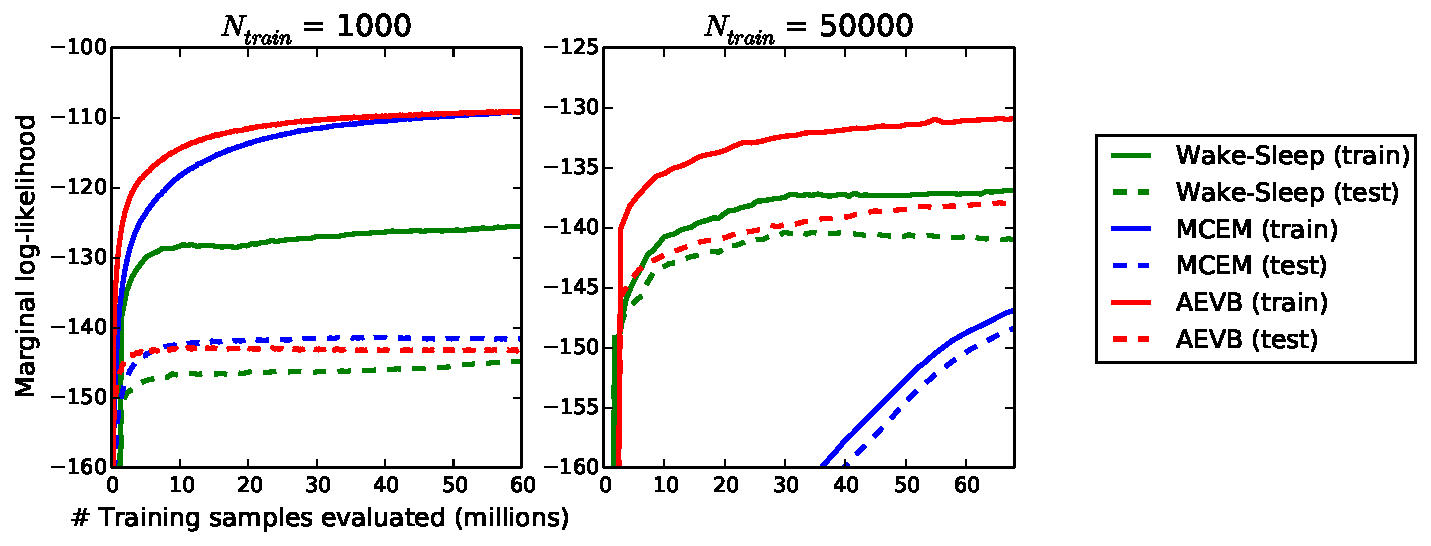
\includegraphics[width=1\columnwidth]{assets/figures/graph_marglik.pdf}

\caption{在不同训练集规模下，根据估计的边缘似然比较 AEVB、唤醒—睡眠算法和蒙特卡洛 EM。蒙特卡洛 EM 不是在线算法，因此与 AEVB 和唤醒—睡眠算法不同，它无法高效地用于完整 MNIST 数据集。
}\label{fig:marglik}
\end{figure}

\paragraph{边缘似然}
当潜在空间维数很低时，可以使用 MCMC 估计量估计学到的生成模型的边缘似然。该估计量的更多信息见附录。编码器和解码器仍采用神经网络，这次使用 100 个隐藏单元和 3 个潜变量；潜在空间维数更高时，估计结果会变得不可靠。这里仍使用 MNIST 数据集。
我们将 AEVB 和唤醒—睡眠方法与采用混合蒙特卡洛（HMC）\cite{duane1987hybrid}采样器的蒙特卡洛 EM（MCEM）进行比较，细节见附录。分别在较小和较大的训练集上比较三种算法的收敛速度，结果见图\ref{fig:marglik}。

\paragraph{高维数据可视化} 若选择低维潜在空间，例如二维空间，就可以用学到的编码器（识别模型）将高维数据投影到低维流形。MNIST 和 Frey Face 数据集的二维潜在流形可视化见附录\ref{ap:visualisations}。
